\chapter{idock 3: protein-ligand docking with GPU acceleration}

\section{Introduction}

\citep{1401} GASPRNG: GPU accelerated scalable parallel random number generator library using CUDA

The modern GPU (Graphics Processing Unit) has evolved from a fixed-function graphics pipeline to a programmable parallel processor with extremely high computational throughput and tremendous memory bandwidth at an affordable price. Performance evaluation of hybrid programming patterns for large CPU/GPU heterogeneous clusters has been carried out \citep{1035}. The past five years have seen a fruitful of algorithms for computer-aided drug discovery being ported to the GPU and gaining orders of magnitude of speedup over single threaded CPU counterparts. To name a few, such GPU-accelerated applications include FTMap \citep{722} for binding site mapping, CUDASW++2.0 \citep{189} for protein database search, the leader and the spread algorithms \citep{750} for compound selection, PIPER \citep{723}, PLANTS \citep{779}, parallelized AutoDock \citep{696}, GPUperTrAmber \citep{1270} and a transcription factor-DNA docking program \citep{1267,1266} for molecular docking, SIML \citep{726} and Tanimoto matrix calculation \citep{881} for chemical similarity calculation, OpenMM \citep{373}, MD-GPU \citep{374} and SPFP \citep{1261} for molecular dynamics, PAPER \citep{491} for molecular shape comparison, gWEGA \citep{1388} for molecular superposition and shape comparison, a k-centers algorithm for clustering conformations \citep{1275}, CAMPAIGN \citep{932} for data clustering, and visualization \citep{986}.

As of October 2012, NVIDIA’s latest GPU architecture is codenamed ``Kepler" with its full implementation codenamed ``GK104", while AMD's latest GPU architecture is codenamed ``Southern Islands" with its full implementation codenamed ``Tahiti".

\subsection{NVIDIA GK104 and CUDA}

From the hardware perspective, the GK104-based GeForce GTX 680 GPU features 3.09 TFLOPS single-precision computing power and 128 GFLOPS double-precision computing power, 2GB GDDR5 memory with a bandwidth of 192GB/s, and a TDP (Thermal Design Power) of 195W.

Figure \ref{GPU:GeForceGTX680BlockDiagram} shows the block diagram of GeForce GTX 680, which consists of 4 GPCs (Graphics Processing Clusters), each having a dedicated raster engine and 2 SMX (next-generation Streaming Multiprocessors) units. With a total of 8 SMX units, the GeForce GTX 680 has 1536 CUDA cores.

\begin{figure}
\centering
%\includegraphics[width=\textwidth]{GPU/GeForceGTX680BlockDiagram.png}
\caption{NVIDIA GeForce GTX680 block diagram. Source: NVIDIA.}
\label{GPU:GeForceGTX680BlockDiagram}
\end{figure}

Figure \ref{GPU:GeForceGTX680SMX} shows the block diagram of GK104 SMX unit, which features 192 IEEE 754-2008 compliant single-precision CUDA cores, 32 SFUs (Special Function Units), 4 warp schedulers, 8 instruction dispatch units, and 64KB of configurable shared memory / L1 cache. Each CUDA core has fully pipelined floating-point and integer arithmetic logic units, while the SFUs handle fast approximate transcendental and graphics interpolation instructions.

The SMX schedules threads in groups of 32 parallel threads called warps. The 4 warp schedulers allow 4 warps to be issued and executed concurrently. Each warp scheduler is capable of dispatching 2 instructions per warp every clock in order to feed the execution resources of SMX.

\begin{figure}
\centering
%\includegraphics[width=\textwidth]{GPU/GeForceGTX680SMX.png}
\caption{NVIDIA GeForce GTX680 SMX. Source: NVIDIA.}
\label{GPU:GeForceGTX680SMX}
\end{figure}

From the software perspective, the GeForce GTX 680 supports CUDA (Compute United Device Architecture), and thus can execute programs written in C, C++, Fortran, and other languages. A CUDA program invokes functions called kernels that execute across parallel CUDA threads, which are organized into thread blocks and grids of thread blocks. The hierarchy of CUDA threads maps to the hierarchy of CUDA cores on the GPU; a GPU executes one or more grids; an SMX executes one or more thread blocks; and CUDA cores and other execution units in the SMX execute thread instructions from kernel compilation.

Figure \ref{GPU:CUDAMemoryHierarchy} shows the CUDA hierarchy of threads, blocks and grids, and their corresponding memory space. A CUDA thread within a thread block maintains a program counter and executes an instance of the kernel. It has a per-thread private memory space used for register spills, function calls, and C automatic array variables. A thread block is a set of concurrently executing threads that can cooperate among themselves through barrier synchronization and shared memory. It has a per-block shared memory space used for inter-thread communication, data sharing, and result sharing. A grid is an array of thread blocks that execute the same kernel, read inputs from global memory, write results to global memory, and synchronize between dependent kernel calls. Grids share results in global memory after kernel-wide synchronization.

\begin{figure}
\centering
%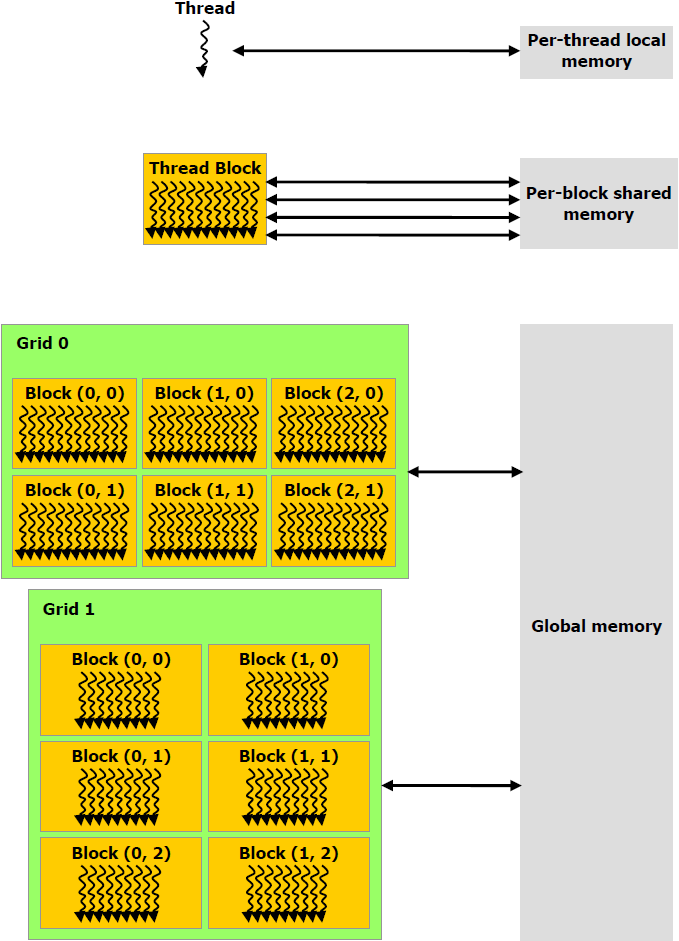
\includegraphics[width=\textwidth]{GPU/CUDAMemoryHierarchy.png}
\caption{CUDA hierarchy of threads, blocks, and grids, with corresponding per-thread private, per-block shared, and per-application global memory spaces. Source: NVIDIA.}
\label{GPU:CUDAMemoryHierarchy}
\end{figure}

\subsection{AMD Tahiti and OpenCL}

From the hardware perspective, the Tahiti-based Radeon HD 7970 GPU features 3.79 TFLOPS single-precision computing power and 947 GFLOPS double-precision computing power, 3GB GDDR5 memory with a bandwidth of 264GB/s, and a TDP of 250W.

Figure \ref{GPU:RadeonHD7970BlockDiagram} shows the block diagram of Radeon HD 7970, which consists of 32 GCN (Graphics Core Next) cores, each heaving 64 stream processors, translating to a total of 2048 stream processors.

\begin{figure}[t]
\centering
%\includegraphics[width=\textwidth]{GPU/RadeonHD7970BlockDiagram.jpg}
\caption{AMD Radeon HD 7970 block diagram. Source: AMD.}
\label{GPU:RadeonHD7970BlockDiagram}
\end{figure}

Figure \ref{GPU:RadeonHD7970GCN} shows the block diagram of GCN core, which features a scheduler, 4 SIMD-16 vector units, 4 64KB vector registers, a single scalar unit, 64KB of LDS (Local Data Share), and 16KB of L1 cache. The GCN core schedules threads in groups of 16 parallel threads called wavefronts. The 4 SIMD-16 vector units are capable of not only processing 4 wavefronts in 4 clock cycles, equivalent to one wavefront per cycle, but also handling special functions like transcendentals at a rate of 4 operations per clock cycle. The scalar unit assists with flow control and handles address generation for pointers. The L1 cache has an aggregate bandwidth of about 2 TB/s.

\begin{figure}
\centering
%\includegraphics[width=\textwidth]{GPU/RadeonHD7970GCN.png}
\caption{AMD Radeon HD 7970 GCN. Source: AMD.}
\label{GPU:RadeonHD7970GCN}
\end{figure}

Figure \ref{GPU:RadeonHD7970CacheHierarchy} shows the cache hierarchy of Radeon HD 7970. A group of 4 GCN cores shares a 16KB instruction cache and a 32KB scalar data cache. The GDS (Global Data Share) enables L1 cache synchronization across all the GCN cores, which communicate over a shared bus to 6 128KB L2 cache partitions, each associated with a 64-bit dual-channel memory controllers, for a total of 768KB of L2 cache. The L2 cache can transfer nearly 710GB/s at 925MHz.

\begin{figure}
\centering
%\includegraphics[width=\textwidth]{GPU/RadeonHD7970CacheHierarchy.jpg}
\caption{AMD Radeon HD 7970 cache hierarchy. Source: AMD.}
\label{GPU:RadeonHD7970CacheHierarchy}
\end{figure}

From the software perspective, the Radeon HD 7970 supports OpenCL (Open Computing Language) 1.2, and thus can execute programs written in C. There is a C++ wrapper for OpenCL 1.1. An OpenCL program invokes functions called kernels that execute across parallel work-items, which are organized into work-groups. The hierarchy of work-items maps to the hierarchy of stream processors on the GPU; a GPU executes one or more kernels; a GCN core executes one or more work-groups; and stream processors execute work-item instructions from kernel compilation.

Portability is the distinct feature that distinguishes OpenCL from CUDA. Multiple conformant implementations of OpenCL from AMD, NVIDIA, Intel, IBM, ARM, and embedded device vendors are shipping, fulfilling the philosophy of ``write once, execute everywhere".

\chapterend
